\documentclass[../report]{subfiles}
\setcounter{section}{0}
\begin{document}

本章では,開発について詳しく説明する.
\bunseki{佐藤碧}


\section{カメラの実装}
本システムでは,動体を自動で検出して写真を撮影し,それをサーバに送信できるようにする必要がある.
それらを実現するためには幾つかの方法が考えられるが,私たちはマイコンの一種であるRaspberry Piを用いることにした.
本システムでは,ボックスにカメラを取り付けて写真を撮影する.
その際,カメラを含めた機器類はなるべく小型であるほうが,カメラを取り付ける際の都合がいい.
例えば,取り付けた際のボックスの外観をシンプルにできるので,取り付けた機器類が目立ちにくくできるのでユーザが不用意に触ることで不具合が起きる事態を防ぎやすいといったことが挙げられる.
また,動体検出,写真撮影,画像の送信といった機能に必要となるリソースは,それほど膨大なわけではない.
よって,通常のコンピュータと比較すると小型である代わりに非力であるRaspberry Piを用いても,必要な機能を実現できると考えた.
以上のような理由から,私たちはRaspberry Piを用いることにした.

動体の自動検出と写真の撮影には,Raspberry PiのパッケージであるMotionを利用する.
MotionはRaspberry Piに接続されたカメラを通して動体を検出して写真を撮影することができるパッケージである.
Motoiinは一度動体を検出すると,動体の検出が終了するまでの間に連続して写真を撮影し続けるといった仕組みになっている.
また,パラメータを変更することによって動体検出の感度を調整することができる.
加えてMotionでは,動体検出で発生するイベントにフックさせて,任意のプログラムを実行させることが可能である.
発生するイベントの内,今回利用したのは以下の3種類である.
\begin{description}
    \item{onEventStart} 動体を検出し,写真を撮影しはじめたとき
    \item{onPictureSave} 動体検出中に写真を撮影して保存したとき
    \item{onEventEnd} 動体検出が終了したとき
\end{description}

Motion自体には写真を送信する機能はないため,上記のイベントにフックさせて実行させるプログラムにてそれを行う.
写真を送信するプログラムはPythonで実装した.
ただし,ここである問題が浮上してくる.
それは,Motionの仕様上,一度の動体検出が発生してから終了するまでの間に,食事が写った写真も写っていない写真も複数撮影されてしまうということである.
そのため,一度の動体検出内で撮影されて写真の中から料理が写っている写真を選択的に送信する必要がある.
この問題を解決するために実装した一連の処理を以下に示す.
\begin{enumerate}
    \item 動体を検出して写真を撮影しはじめたとき(onEventStart)に,その時点の日付と時間を元にしたテキストファイルを作成する.
    \item 動体検出中に写真を撮影して保存する(onPictureSave)たびに,1.で作成したテキストファイルに保存したファイル名を書き込む.
    \item 動体検出が終了したとき(onEventEnd)に,1.で作成したテキストファイルから食事が写っている写真のファイル名を取得して,その写真をサーバに送信する.
\end{enumerate}
なお,1.でテキストファイルを作成するのは,Motionの仕様上撮影された写真は保存先として一つのディレクトリしか指定できないため,一回の動体検出イベントで撮影された写真を識別することができないからである.
また,テキストファイルの名前を日付と時間をもとに決めるのは,最新の動体検出イベントによって作成されたテキストファイルを識別するためである.
これにより,3.ではテキストファイルが保存されているディレクトリ内のファイルを,名前でソートすることで最新の動体検出イベントで撮影された写真を識別することが可能となる.
この方法によって撮影された写真のファイル名が書き込まれたテキストファイルを取得し,その中からファイルの中盤に書かれている写真のファイル名を,写真を送信するプログラムに渡してサーバに送信する.
テキストファイルには一回の動体検出によって保存された写真のファイル名が保存されて順番に保存されているが,そのうち中盤のものを選択して送信するのは,Motionの特性上食事の写った写真である可能性が高いと考えられるからである.
と言うもの,Motionは動体検出ができるが,その検出が終了するのはカメラに動体が映らなくなってからある程度時間が経ってからだからである.
そのため,テキストファイルの序盤に保存された写真には動体検出が始まってから,料理がボックス内に置かれている最中の様子が,中盤には料理がボックス内に置かれてから手が引き抜かれるまでの様子が,終盤には手が引き抜かれてからMotionの動体検出が終了するまでの様子が写っていると考えられる.
よってテキストファイルの中から中盤のものを選択して送信すれば,料理の写っている写真が送信できるのである.

Motionは上記でも述べたように動体検出ができる.
しかし,ここで一つの問題が浮上してくる.
それは,Motion自体はボックス内に食事を置く際でも取り出す際でも,等しく動体検出を行い写真を撮影してしまうということである.
したがって,単純に動体検出が終了した際に最後に撮影した写真を送信するという処理を行うと,ボックス内に食事を置いた際はきちんと写真が撮影されてそれがサーバに送信されるが,ボックス内から食事を取り出した際にも同様に写真が撮影されサーバに送信されてしまう.
つまりは,本来不要な写真がサーバに送信されてしまうということである.
この問題に対しては,2つの解決方法が考えられる.
一つは,写真が送信されるサーバ側で写真の選別を行い,必要とされる写真だけを利用するようにする方法である.
もう一つは,写真を送信する前にRaspberry Pi内で写真の選別を行い,必要となる写真だけをサーバに送信するという方法である.
今回は,後者の方法を取ることにした.
理由は,可能であるのなら,問題はその問題が起きている範囲で解決できたほうが複雑にならなくて済むからである.
写真の選別は背景差分法を用いて行う.
背景差分法とは,物体が写っているか調べたい画像と事前に背景用として用意しておいた画像とをピクセル単位で比較し,相違点が多ければ物体が写っていると判断し,そうでなければ物体は写っていないと判断するといった手法である.
実装はPythonと画像処理ライブラリであるOpenCVを用いて行った.

このようにして,上記の問題の解決を図った.
しかし残念ながら,精度はまだまだ甘く一定の効果は認められたものの,実際には本来送信するべきでない料理が写っていない写真を送信してしまうことがある.
原因としては,ボックス内に写り込んでしまう影が考えられる.
背景差分法は,2枚の画像同士をピクセル単位で比較している.
そのため,影が写り込んだ写真とそうでない写真を比較した場合,特にそれが食事が写っていない写真である際には,画像同士の相違点が多いと判断されてしまい,結果食事が写っていない写真にも関わらず,その写真が送信されてしまうといったことが起きてしまう.
したがって,サーバに食事が写っていない写真が送信されてしまうといった問題は解決できたとはいえない.
解決するためには,画像の些細な変化に対応できるような,いわゆる揺らぎを許容出るようなアルゴリズムの採用,あるいは,機械学習を用いた画像認識を利用するといったことが考えられる.
今回は時間や実装を担当したメンバーの技術力不足によってこの問題を解決し切ることができなかった.
よってこの問題は,今後の解決するべき課題として挙げられる.
\bunseki{佐藤碧}


\section{ボックスの実装}
\bunseki{佐藤碧}


\section{Webサーバの実装}
Webサーバの実装には,RubyのWebフレームワークであるRuby on Railsを使用した.
Webフレームワークの使用に至った経緯は,3.2.2に示した.
ユーザには1人1アカウントが割り当てられ,それぞれ閲覧できる・閲覧されるユーザが指定できるよう多対多のリレーションを構築した.

ユーザーが箱を通して送る毎日の食事の画像は,本サーバを経由してAmazon S3に保存される.
また,食事の画像が保存されると同時にジョブがキュー上に登録され,順に料理画像認識が実行される.
この画像認識は別のAPIサーバ上で実行され,その実装については6.3に記す.
APIサーバから画像認識の結果が返ってくると,食事と料理の紐付けが保存される.

料理とその料理の一般的な栄養価の対応表は,あらかじめデータベースに用意しておき,画像認識で返ってくる料理名と一致することで,カメラに写った食事の栄養価が分かるというような実装とした.
また用意したデータベースに認識結果の料理名のものが入っていない場合は,ユーザーがウェブブラウザを介して登録できるようにした.

フロントエンドでは,見た目を整えるためにBootstrap4を使用した.また一部動的なコンテンツを実装するためにVue.jsを使用した.
TV画面の実装には,リアルタイムに撮影された食事画像や家族・医療従事者からのコメントが表示されるようにWebSocketを使用し,Vue.jsを通して表示している.
過去の食事画像やコメントは,RailsのJSON Builderを使用して,フロントエンドからJSONとして受け取れるようにしている.
\bunseki{佐藤礼於}


\section{料理画像認識の実装}
料理画像の認識には3.2.3で示したように「docomo 画像認識API」を使用している.
このWebAPIは一つの画像につき一つの物体のみの認識に特化しており,複数の食事が写った画像を入力に使用しても全体を一つの料理として捉えて結果を返す.
今回のシステムでは複数の料理を箱に入れても正常に認識が行えることが理想であるため,これを実現するには皿ごとに画像を分け,その皿の枚数だけ「docomo 画像認識API」に入力として与える必要がある.
私達はOpenCVを使用して二値化閾値処理を行い,皿の範囲を割り出すこととした.
今回のプロダクトでは白い箱を使用するので,背景は常に白であるから,閾値による皿の判別は比較的容易であった.
閾値で皿を識別した後,輪郭を抽出することで皿の判定が可能となった(図\ref{fig:6-threshold}).

\begin{figure}[htbp]
    \begin{center}
        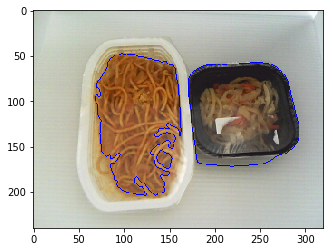
\includegraphics[width=10cm]{imgs/6-threshold.png}
        \caption{閾値によって皿を識別}
        \label{fig:6-threshold}
    \end{center}
\end{figure}

今回は皿ごとの画像に分ける必要があるため,輪郭から外接矩形を検出し,元の画像から皿ごとの画像に切り分けることとした(図\ref{fig:6-bounding}).

\begin{figure}[htbp]
    \begin{center}
        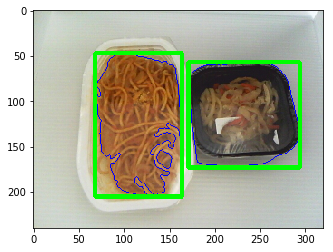
\includegraphics[width=10cm]{imgs/6-bounding.png}
        \caption{外接矩形で皿を囲む}
        \label{fig:6-bounding}
    \end{center}
\end{figure}

皿ごとの画像に切り分けることができたこれらを「docomo 画像認識API」に入力として与えると,複数の候補がJSONで返却される.

本システムでは,最もスコアの高い認識結果をその皿の料理名としてウェブサーバに保存するようにしている.
\bunseki{佐藤礼於}

\end{document}
